\chapter{Analytisk Mekanik}
%
%
\section*{Koordinatsystemer}
\begin{opgave}{Gode koordinatsystemer}{1}
At få valgt et smart koordinatsystem er essentielt i analytisk mekanik.
\opg Beskriv hvad der kendetegner et smart valg af koordinatsystem?
\opg Hvorfor kan det smarte koordinatsystem identificeres ud fra symmetri?
\opg Hvilket koordinatsystem er smartes for et problem med: \\
a) Plansymmetri. \\
b) Cylindrisk symmetri. \\
c) Sfærisk symmetri. \\
Forklar hvorfor?
\end{opgave}
%
%
\begin{opgave}{Generaliserede koordinater}{1}
Betragt et objekt der er fanget på en ring med centrum i origo, $(0,0)$, og radius $R$.
\opg Definer et sæt polære koordinater $(r,\phi)$, og skriv de kartesiske koordinater op med disse.
\opg Hvor mange af de kartesiske koordinater ændres, når objektet bevæger sig på ringen?
\opg Hvor mange af de polære koordinater ændres, når objektet bevæger sig på ringen?
\opg Hvor mange koordinater skal der bruges for at beskrive objektets bevægelse?
\opg Hvad er det smarte koordinatvalg?
\end{opgave}
%
%
\begin{opgave}{Brint}{2}
Hydrogenisotopen $^1$H består af en proton med massen $m_p$ og ladningen $e$ (elementarladningen), samt en elektron med massen $m_e$ og ladningen $-e$. Fra elektrostatik\footnote{Elektrostatik er studiet af elektriske felter dannet af stillestående (statiske) elektriske ladninger.} oplyses det, at kraften fra en punktladning $Q_1$ med stedvektor $\v{r}_1$ på en punktladning $Q_2$ med stedvektor $\v{r}_2$ er
\begin{align} \label{eq:F_el}
	\v{F} = \frac{Q_1Q_2}{4\pi\epsilon_0}\frac{\v{r}_2-\v{r}_1}{|\v{r}_2-\v{r}_1|^3} \: ,
\end{align}
hvor $\epsilon_0$ er en konstant, der kaldes vakuumpermittiviteten. Punktladninger er ladninger uden udstrækning, hvorfor de eksisterer i ét punkt i rummet og kun det punkt. Elektroner og protoner er så små, at de kan beskrives som punktladninger, hvorfor ligning \eqref{eq:F_el} kan benyttes.
\opg Skitser situationen og indtegn systemets massemidtpunkt. Hint: Se formel (\ref{CM}) for definitionen af massemidtpunktet (på engelsk center of mass, forkortes CM).
\opg Hvad betyder $|\v{r}_2-\v{r}_1|$ fysisk?
\opg Indtegn kræfterne på begge ladninger i jeres tegning.
\opg Hvor er det smartest at placere origo? \\ \\
Massemidtpunktet for et tolegemesystem er defineret som
\begin{align}
\label{CM}
	\v{r}_\textsc{cm} = \frac{m_1\v{r}_1 + m_2\v{r}_2}{m_1 + m_2} \, .
\end{align}
\opg Hvad bliver $\v{r}_{\textsc{cm}}$ for vores system under approksimationen at $m_p \gg m_e$?
\opg Opskriv kraften på elektronen i dette koordinatsystem.
\end{opgave}
%
%
\section*{Energi}
%
%
\begin{opgave}{Energibevarelse}{1} \label{opg:Energibevarelse}
Energi er altid bevaret. Den kan omdannes mellem forskellige former, men den forsvinder aldrig.
\opg Opskriv nogle af de typer af energi, som du kan komme på.
\opg Forklar i egne ord hvad en konservativ kraft er.
\opg Summen af kinetisk og potentiel energi kaldes mekanisk energi, og er bevaret i et system, så længe det kun er påvirket af konservative kræfter. Angiv tre eksempler på systemer, hvor den mekanisk energi er bevaret, og tre hvor den ikke er.
\opg Angiv for hvert eksempel hvor den mekaniske energi ikke er bevaret, hvad årsagen er til dette.
\end{opgave}
%%
%%
\begin{opgave}{Frit fald}{1} \label{opg:FritFald}
Et legeme med massen $m$ frigives fra hvile i en afstand $h$ over Jordens overflade. Antag at tyngdeaccelerationen er konstant og har værdien $g$.
\opg Tegn et kraftdiagram for systemet.
\opg Hvorfor er den mekaniske energi ikke bevaret?
\opg Negliger nu den kraft der ødelægger energibevarelsen, og bestem legemets fart i det øjeblik det rammer Jorden.
\opg Diskuter hvor god en antagelse det er at negligere den "problematiske"\;kraft, og opstil et muligt kriterie for, at det er en god antagelse negligere denne.
\end{opgave}
%
%
\begin{opgave}{Kollisioner}{1}
Når to legemer kolliderer kan det inddeles i to grupper: elastiske og uelastiske kollisioner. Under kollisionen påvirker legemerne hinanden med en eller flere kræfter, og elastiske kollisioner defineres som kollisioner, hvor disse kræfter udelukkende er konservative. Der ses bort fra eventuelle ydre kræfter.
\opg Hvorfor er størrelsen af den samlede kraft fra legeme 1 på legeme 2, den samme som den samlede kraft fra legeme 2 på legeme 1?
\opg I hvilken retning går kraften på legeme 2 i forhold til kraften på legeme 1?
\opg Benyt Newtons anden lov til at vise, at systemets totale impuls er bevaret.
\opg Er den kinetiske energi bevaret for en \\
a) Elastisk kollision? \\
b) Uelastisk kollision?\\
\end{opgave}
%
%
\begin{opgave}{Bevægelse omkring ligevægt}{2}\label{mek:opg:equilibrium}
Det antages, at en masse $m$ er påvirket af den sfærisk symmetriske\footnote{Sfærisk symmetri i den potentielle energi betyder her, at det kun er massens afstand til nulpunktet, der betyder noget for den potentielle energi, men ikke hvor på sfæren med radius $r$ den er.} potentielle energi
\begin{align*}
V(r) = V_0\left(\frac{r}{R} + \lambda^2\frac{R}{r}\right) \, ,
\end{align*}
hvor $V_0,R,\lambda$ alle er positive konstanter.	Massens bevægelse omkring ligevægtspunktet ønskes nu undersøgt. \\
\opg Bestem den afledede af den potentielle energi $V(r)$, i forhold til $r$. Dvs. $\text{d}V / \text{d} r$.
\opg Bestem afstanden $r_0$, hvor $\d V/\d r = 0$.
\opg Find den andenafledede $\text{d}^2 V / \text{d} r^2$.
\opg Argumenter for at $r_0$ er det punkt, hvor den potentielle energi er mindst, altså at potentialet stiger, hvis $r$ afviger fra $r_0$.
\opg Nu defineres $x$ som afstanden, regnet med fortegn, fra $r_0$, det vil sige $x = r - r_0$. Udtryk den potentielle energi ved $x$, altså $V(x)$.
\opg Vis at den potentielle energi, $V(x)$, har formen for en harmonisk oscillator (periodisk svingning) for små $x$. \\
Hint: Vis at en Taylorudvikling til anden orden giver en potentiel energi på formen
\begin{align*}
	V(x) = c + \frac{1}{2}kx^2 \, ,
\end{align*}
hvor $c$ og $k$ er konstanter. 
\opg Bestemt vinkelfrekvensen for massens oscillationer under denne approksimation. \\
Hint: Under denne approksimation opfører systemet sig som en harmonisk oscillator analogt til klodsen på fjederen i afsnit \ref{k-sec:fjeder} i kompendiet.
\end{opgave}
%
%
\begin{opgave}{(Næsten) alt er en harmonisk oscillator}{3} \label{opg:HO}
En harmonisk oscillator har potentiel energi på formen $f(x) = c + \frac{1}{2}kx^2$, hvor $c$ og $k$ er konstanter. Betragt nu et arbitrært, endimensionelt system med potentiel energi $V(x)$, hvor $x$ er det generaliserede koordinat. Det vil sige, at $V(x)$ er en ukendt funktion, vilkårlig funktion\footnote{Dette skal forstås som at vi intet ved om den, fordi det resultat vi opnår så gælder for enhver funktion.}.
\opg Med henvisning til tabel \ref{k-Taylorseries_table} i kompendiet, opskriv Taylorpolynomiet til 2. orden for $V$ omkring punktet $x=0$.
\opg Hvad er kriteriet for, at systemet til 2. orden er en harmonisk oscillator?
\opg Giv eksempler på funktioner der opfylder kriteriet. \\ 
I eksemplerne er det gentagende gange benyttet, at nulpunktet for den potentielle energi kan vælges frit. Dette vil være smart at vise. \\
Lad derfor $V(x)$ være den potentielle energi fra før, og $\tilde{V}(x) = V(x) + \lambda$, hvor $\lambda$ er en konstant, være en ny potentiel energi. I Newtons formulering af mekanikken bestemmer kræfter legemers bevægelse, hvor det i Lagrangeformalismen er Euler-Lagrangeligningen. I begge tilfælde er det de afledede med hensyn til sted, der bestemmer, hvordan systemet opfører sig.
\begin{align}
	&\mathrm{Newton:} \qquad\qquad\quad\enspace F = -\pdif{x}{V} \label{eq:V_i_Newton} \\[1em]
	&\mathrm{Lagrange:} \enspace 
	\begin{aligned}
	\el{\dt{x}} &= \pdif{x}{L} \\
	\Rightarrow \dif{t}{}\left(\pdif{\dt{x}}{K}\right) &= \pdif{x}{K} - \pdif{x}{V}
	\end{aligned} \label{eq:V_i_Lagrange}
\end{align}
%hvor implikationen gælder, fordi den potentielle energi ikke afhænger af $\dt{x}$.
\opg Vis at begge potentielle energier $V(x)$ og $\tilde{V}(x)$, giver den samme fysik, dvs. ligningerne er ens.
\opg Brug dette til at vise at fysikken ikke ændrer sig ved at droppe 0. ordens ledet i Taylorpolynomiet. Med andre ord, vis at $V(x) \simeq c + \frac{1}{2}kx^2$ og $V(x) \simeq \frac{1}{2}kx^2$  opfører sig ens overfor ligningerne \eqref{eq:V_i_Newton} og \eqref{eq:V_i_Lagrange}.
\end{opgave}
%
%
\section*{Etlegemeproblemer}
%
%
\begin{figure}[h!]
\centering
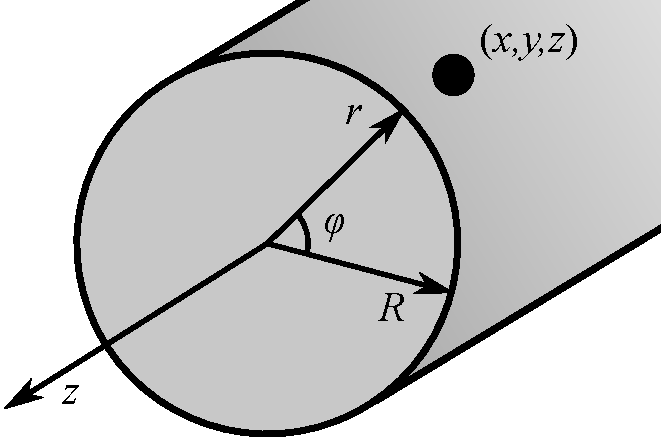
\includegraphics[width = .72\columnwidth]{Analytisk-Mekanik/cylinderopg_sh.pdf}
\caption{Partikel på cylinder.} \label{cyl-fig}
\end{figure}
%
%
\begin{opgave}{Partikel på en cylinder}{1} \label{opg:Cylinder}
Vi ser på en partikel, der kan bevæge sig frit på overfladen af en cylinder med radius $R$, som det ses på figur \ref{cyl-fig}. Her er det oplagt at bruge cylindriske koordinater:
\begin{align*}
x &= r\cos(\phi) \, , \\
y &= r\sin(\phi) \, , \\
z &= z \, .
\end{align*}
\opg Brug de cylindriske koordinater som generaliserede koordinater. Hvilke koordinater ændres, når partiklen bevæger sig?
\opg Udregn $\dt x$, $\dt y$ og $\dt z$ i de nye koordinater.
\opg Opstil den kinetiske energi, $K=\frac{1}{2}mv^2$.
\opg Opstil Lagrangefunktionen. Den potentielle energi er altid nul.
\opg Brug Euler-Lagrangeligningerne til at opstille anden ordens differentialligninger, for de koordinater der ændres, når partiklen bevæger sig.
\opg Hvordan bevæger partiklen sig?
\end{opgave}
%
%
\begin{figure}[h!]
	\centering
	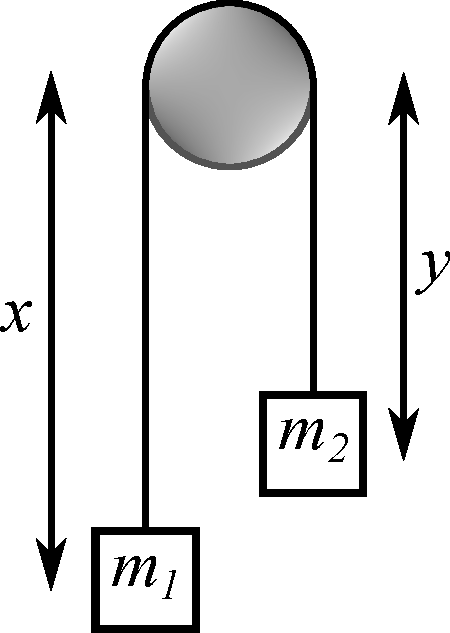
\includegraphics[width=.65\columnwidth]{Analytisk-Mekanik/Atwood.pdf}
	\caption{Illustration af Atwoods faldmaskine, hvor to lod forbindes med en snor over en trisse.} \label{fig:Atwood}
\end{figure}
%
%
\begin{opgave}{Atwoods faldmaskine}{1} \label{opg:Atwood}
I figur \ref{fig:Atwood} ses en illustration af Atwoods faldmaskine, hvori to lodder hænges i hver sin ende af en snor med konstant længde $l$. I figuren er to koordinater også defineret, og de to lodders masser er indtegnet.
\opg Argumenter for at der kun er ét generaliseret koordinat, og udtryk $y$ ved $x$.
\opg Udtryk $\dt{y}$ ved $\dt{x}$.
\opg Definer hhv. $x = 0$ og $y = 0$ som nulpunkt for den potentielle energi for hvert lod, og opskriv den totale potentielle energi\footnote{Har man svært ved at acceptere gyldigheden af at regne med negativ potentiel energi, kan man godt definere nulpunktet under faldmaskinen, hvilket gør at Lagrangefunktionen kommer til at indeholde nogle ekstra konstanter.}.
\opg Opskriv den kinetiske energi som summen af den kinetiske energi for hver af de to lodder.
\opg Vis at Lagrangefunktionen for systemet kan skrives på formen
\begin{align*}
	L(x,\dt{x},t) &= \frac{1}{2}(m_1+m_2)\dt{x}^2 \\
	&+ g\Big(m_1x + m_2(l-x-\pi R)\Big) \: .
\end{align*}
\opg Vis ved brug af Euler-Lagrangeligningen, at systemets bevægelsesligning er
\begin{align*}
	\ddt{x} = g\frac{m_1-m_2}{m_1+m_2} \: .
\end{align*}
\opg Vis ud fra bevægelsesligningen, hvad fortegnet af $\ddt{x}$ er afhængigt af om $m_1>m_2$ eller $m_2>m_1$. Hvilket af de to lodder vil falde ned (hvad betyder det for retningen af bevægelsen)?\\ 
Skrives bevægelsesligningen lidt om fås
\begin{align*}
	\dif[2]{t}{x} &= g\frac{m_1-m_2}{m_1+m_2} = a \\
	\implies \dif{t}{} \left( \dif{t}{x} \right) &= a \\
	\implies \dif{t}{x} &= \ubint{a}{t}\\
	\implies x(t) &= \ubiint{a}{t}{t}
\end{align*}
Det trick vi bruger her er, at integration og differentiation er hinandens omvendte operationer ligesom plus og minus er hinandens omvendte operationer.\footnote{Faktisk har vi også antaget, at to integrationskonstanter er $0$, men det er en mindre detalje.} 
\opg Bestem $x(t)$ ved ovenstående integral.\\ 
Hint: Regn det inderste integrale, så det yderste.
\end{opgave}
%
%
\begin{opgave}{Yoyo}{1} \label{opg:Yoyo}
Betragt yoyoen i figur \ref{fig:yoyo} med massen $m$ og de fysiske dimensioner som vist i figuren.
%
\begin{figure}[]
	\centering
	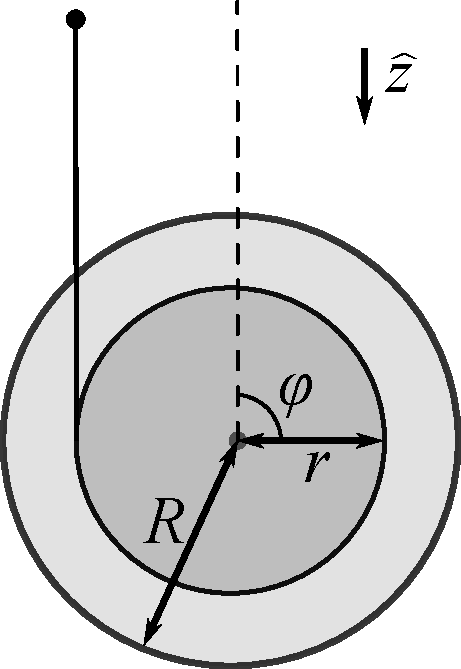
\includegraphics[width=.61\columnwidth]{Analytisk-Mekanik/yoyo.pdf}
	\caption{Skitse af en simpel yoyomodel med radier $r$ og $R$ i et tyngdefelt med i nedadgående retning med styrken $g$.} \label{fig:yoyo}
\end{figure}
%
Tyngdekraften har størrelsen $g$ i $z$-retningen, $\v{F}_\mathrm{g} = mg\zhat$, og den ideelle snor sidder fast i afstanden $r$ fra centrum. At snoren er ideel betyder, at den anses som ustrækkelig, masseløs, og derudover anses friktionen mellem snoren og yoyoen som værende så stor, at yoyoen ikke glider. Det kan vises, at yoyoens inertimoment i denne model er
\begin{align*}
	I = \frac{1}{2}mR^2 \: .
\end{align*}
Som generaliseret koordinat benyttes $z$, fordi $z$ og $\phi$ er koblede.
\opg Antagelsen at friktionen mellem snoren og yoyoen er tilpas stor, gør at det punkt hvor snoren slipper yoyoen står stille, hvilket betyder, at rotationen lige præcis udligner bevægelsen fra, at yoyoen falder nedad.\footnote{Dette kaldes ofte at yoyoen \textit{ruller uden at glide}, hvilket er en meget almindelig antagelse i fysik.} Det betyder, at farten $v$ i ligning \eqref{k-eq:SmartFart} er lig med farten $v_\textsc{cm}$ i ligning \eqref{k-eq:K}, hvor begge ligninger henviser til kompendiet. Brug disse ligninger til at vise at
\begin{align*}
	K = \frac{1}{2}m\dt{z}^2 + \frac{1}{4}mR^2\left(\frac{\dt{z}}{r}\right)^2 \: .
\end{align*}
\opg Argumenter for at den potentielle energi kan skrives på formen $V = -mgz$.
\opg Konkluder at Lagrangefunktionen for problemet er
\begin{align*}
	L = \frac{1}{2}m\left[1 + \frac{1}{2}\left(\frac{R}{r}\right)^2\right]\dt{z}^2 + mgz \: .
\end{align*}
\opg Bestem nu følgende afledede af Lagrangefunktionen
\begin{align*}
	\pdif{z}{L} &= \; ? \\
	\pdif{\dt{z}}{L} &= \; ? \\
	\el{\dt{z}} &= \; ?
\end{align*}
\opg Brug Euler-Lagrangeligningen, ligning \eqref{k-Euler-Lagrange} i kompendiet, til at vise at
\begin{align} \label{eq:YoyoDiffLign}
	\ddt{z} = \frac{g}{1 + \frac{1}{2}\left(\frac{R}{r}\right)^2} \: .
\end{align} \\[1mm]
Det kan vises at løsningen til denne differentialligning er
\begin{align} \label{eq:YoyoBevLign}
	z(t) = \frac{g}{2}\left[1 + \frac{1}{2}\left(\frac{R}{r}\right)^2\right]^{-1}t^2 + v_0t + z_0 \: ,
\end{align}
hvor $v_0$ er startfarten, og $z_0$ er startstedkoordinatet. Ved indsættelse i ligning \eqref{eq:YoyoDiffLign} kan det vises, at ligning \eqref{eq:YoyoBevLign} er en løsning, eller det kan udledes med samme metode som i opgaverne \ref{opg:Atwood} og \ref{opg:cylinder}.
\opg Overvej hvilke fordele og ulemper der er, ved at benytte Lagrangemekanikken til at løse dette problem frem for Newtonsk mekanik.
\end{opgave}
%
%
\begin{opgave}{Klods på en fjeder}{2}
I starten af kompendiets første kapitel blev det vist, at bevægelsesligningen for en klods på en fjeder, figur \ref{k-fig:fjeder} i kompendiet, er
\begin{align*}
	\ddt{x} = -\frac{k}{m}x \: .
\end{align*}
Til dette blev Newtons formulering af mekanikken brugt, men det samme kan også opnås med Lagrangeformalismen.
\opg Opstil Lagrangefunktionen for problemet.
\opg Benyt Euler-Lagrangeligningen til at komme frem til det samme.
\end{opgave}
%
%
\begin{opgave}{Cylinder på skråplan}{2}\label{opg:cylinder}
En cylinder med massen $m$, radius $R$ og inertimoment $I$ placeres på et skråplan med vinklen $\alpha$ i forhold til vandret.\\
\opg Skitser situationen.
\opg Indtegn på skitsen det koordinatsystem, der giver det færrest mulige afhængige koordinater.
\opg Opstil den potentielle energi $V$ for systemet, hvor der ses bort fra cylinderes udtrækning.
\opg Udtryk den kinetiske energi $K$ ved cylinderens fysiske parametre og tidsafledede af de valgte generaliserede koordinater.
\opg Opskriv problemets Lagrangefunktion.
\opg Vis at ved løsning af Euler-Lagrangeligningen fåes
\begin{align*}
\ddt{x} = -\dfrac{g\sin\alpha}{1+I/mR^2} \: .
\end{align*}
\opg Argumenter for at accelerationen er konstant.
\opg Lad nu accelerationen være $\tilde{g}$, og vis at bevægelsesligningens løsning er
\begin{align*}
x(t) = \frac{1}{2}\tilde{g}t^2 + v_0t + x_0 \: .
\end{align*}
\end{opgave}
%
%
\begin{figure}[h!]
	\centering
	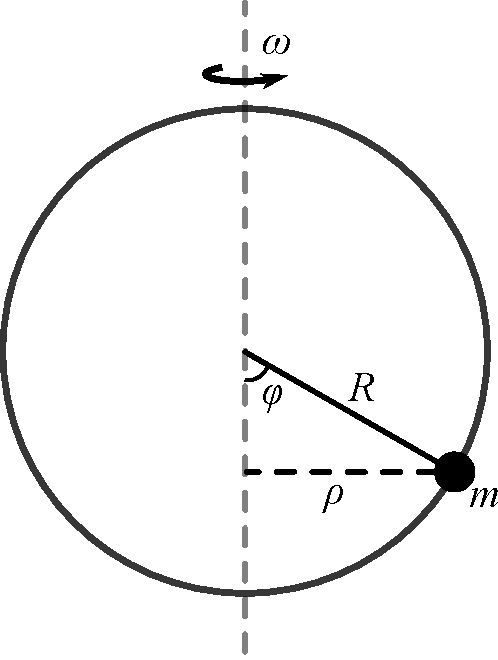
\includegraphics[width=.65\columnwidth]{Analytisk-Mekanik/BeadOnHoop.pdf}
	\caption{Illustration af situationen, hvor koordinater og andre parametre er indtegnet.} \label{fig:BeadOnHoop}
\end{figure}
%
%
\newpage
\begin{opgave}{Masse på roterende ring}{3}
Et lod med masse $m$ er placeret på en ring, hvorpå den kan bevæge sig friktionsløst, som i figur \ref{fig:BeadOnHoop}. Ringen har radius $R$, og den roterer om sin egen akse med vinkelhastigheden $\omega$. Massen kan beskrives udelukkende ved det generaliserede koordinat $\phi$, men for at indse dette gøres brug af koordinatet $\rho$.
\opg Udtryk den potentielle energi ved det generaliserede koordinat $\phi$, således at $V(\phi=0)=0$.
\opg Massens hastighed deles nu op i to komponenter - en der svarer til ind i tegningen og en langs ringen. Disse kaldes henholdsvis $v_\mathrm{ring}$, idet det er bevægelsen som følge af ringens rotation, og $v_\mathrm{lod}$ idet det er lodets bevægelse på ringen. Bestem disse komponenter udtrykt ved $\omega$, $\phi$ og $\dt{\phi}$, samt eventuelle geometriske parametre.\\
Hint: Benyt ligning \eqref{k-eq:SmartFart} i kompendiet.
\opg Brug dette til at bestemme den kinetiske energi, og vis dermed at Lagrangefunktionen er
\begin{align*}
	L = \frac{1}{2}mR^2\big[\dt{\phi}^2 + \omega^2\sin^2(\phi)\big] - mgR\big[1-\cos(\phi)\big] \: .
\end{align*}
\opg Benyt Euler-Lagrangeligningen til at vise, at bevægelsesligningen er
\begin{align*}
	\ddt{\phi} = \left[\omega^2\cos(\phi) - \frac{g}{R}\right]\sin(\phi) \: .
\end{align*}
\opg Hvad er kriteriet for henholdsvis et stabilt og ustabilt ligevægtspunkt fysisk og matematisk?
\opg Brug kriterierne til at bestemme systemets ligevægtspunkter, og forklar hvad de betyder fysisk.
\opg Eksister alle disse punkter for alle $\omega, R$ og $g$?
\opg Diskuter om ligevægtspunkterne er stabile eller ustabile i alle tilfælde fra sidste spørgsmål.\footnote{Ligevægtspunkterne $\phi_0 = 0,\pm\pi$ er ikke super komplicerede at vise stabiliteten af matematisk, men det sidste er svært, hvorfor dette bør tilgås med forsigtighed. Det er dog vist i facitlisten, hvordan dette gøres, hvilket kan være en gennemlæsning værd.}
\end{opgave}
%
%
\section*{Flerlegemeproblemer}
%
%
\begin{figure}[h!]
\centering
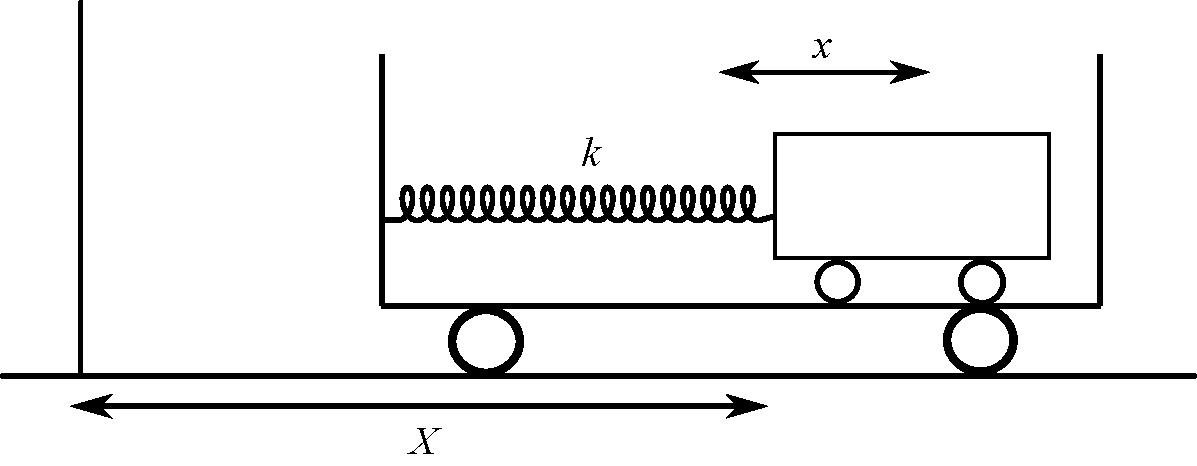
\includegraphics[width=\columnwidth]{Analytisk-Mekanik/ToKobledeVogne.pdf}
\caption{Illustration af problemet i opgave \ref{opg:ToKobledeVogne}. $X$ er stedkoordinatet for den store vogn, og $x$ er stedkoordinatet for den lille, hvor $x=0$ defineres som midtpunktet i den store vogn.}
\label{fig:ToKobledeVogne}
\end{figure}
%
%
\begin{opgave}{To koblede vogne}{2} \label{opg:ToKobledeVogne}
En lille vogn med massen $m$ placeres i en større vogn, og de to forbindes med en fjeder med fjederkonstant $k$. Den lille vogn antages at kunne bevæge sig friktionsløst i forhold til den store og den store i forhold til underlaget, og de generaliserede koordinater defineres som på figur \ref{fig:ToKobledeVogne}. Den store vogn tvinges til simpel harmonisk bevægelse, det vil sige $X = A\cos(\omega t)$, hvor $A,\omega$ er konstanter, og derudover kaldes den lille vogns naturlige vinkelfrekvens $\omega_0 = \sqrt{\frac{k}{m}}$.
\opg Argumenter for at den lille vogns hastighed i forhold til underlaget kan skrives som
\begin{align*}
v = \dt{x} + \dt{X} \: ,
\end{align*}
og brug dette til at indse, at
\begin{align*}
K = \frac{1}{2}m\left(\dt{x} + \dt{X}\right)^2 \: .
\end{align*}
\opg Argumenter for at den potentielle energi for den lille vogn er
\begin{align*}
V = \frac{1}{2}kx^2 \: ,
\end{align*}
og konkluder at
\begin{align*}
L = \frac{1}{2}m\left(\dt{x} + \dt{X}\right)^2 - \frac{1}{2}kx^2 \: .
\end{align*}
\opg Brug dette til at vise, at
\begin{align*}
\pdif{\dt{x}}{L} &= m(\dt{x} + \dt{X}) \: ,\\
\pdif{x}{L} &= -kx \: .
\end{align*}
\opg Vis at
\begin{align*}
\dif{t}{}\left(\pdif{\dt{x}}{L}\right) = m\ddt{x} - Am\omega^2\cos(\omega t) \: ,
\end{align*}
og konkluder at
\begin{align*}
\ddt{x} + \frac{k}{m}x = A\omega^2\cos(\omega t) \: .
\end{align*}
\opg Fastholdes den store vogn nu i $X=0$ bliver systemet i denne opgave ækvivalent til et system, uden den store vogn, hvor fjederen på den lille vogn er spændt fast på væggen, hvilket er en harmonisk oscillator. $X=0$ kan realiseres ved at sætte $A=0$. Vis at bevægelsesligningen i dette tilfælde reducerer til en harmonisk oscillator.
\opg Hvorfor er det relevant at tjekke at systemet reducerer til en harmonisk oscillator i grænsen $A=0$?\\ \\
\end{opgave}
%
%
\begin{figure}[h!]
\centering
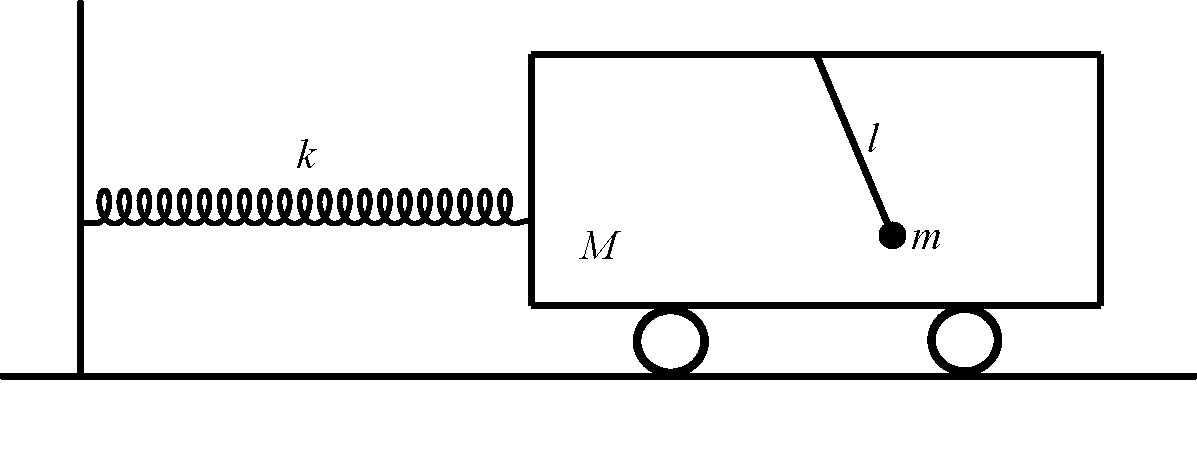
\includegraphics[width=\columnwidth]{Analytisk-Mekanik/PendulIVognOpg.pdf}
\caption{Pendul med massen $m$ og længden $l$ placeret i en vogn med massen $M$, der er fastgjort til en væg med en en fjeder med fjederkonstant $k$.}
\label{fig:PendulIVognOpg}
\end{figure} 
%
%
\begin{opgave}{Pendul i en vogn}{4}
I figur \ref{fig:PendulIVognOpg} er der tegnet et pendul, ophængt i en vogn, der tilmed er fastspændt med en fjeder til en væg, og de relevante fysiske størrelser er indtegnet.
\opg Identificer systemets generaliserede koordinater, indtegn enhedsvektorerne for et kartesisk koordinatsystem og definer origo. %(hint: Se beskrivelsen af pendulet med Lagrangeformalismen og opgave \ref{opg:ToKobledeVogne})
\opg Opskriv pendulets kartesiske koordinater, $(X_p,Y_p)$, udtrykt ved de generaliserede koordinater, samt vognens kartesiske $X$-koordinat, $X_v$, og argumenter for, at $Y_v$ er ubetydelig for problemet.
\opg Bestem systemets potentielle energi.
\opg Bestem systemets kinetiske energi og opskriv Lagrangefunktionen. %(hint: Anvend de kartesiske koordinater fra sidste opgave til først at bestemme de relevante hastigheder)
\opg Vis at løsningen til Euler-Lagrangeligningen er de koblede differentialligninger
\begin{align*}
a&) \quad M\ddt{x} + m\ddt{x} + ml\ddt{\phi}\cos\phi - ml\dt{\phi}^2\sin\phi = -kx \:, \\
b&) \quad ml^2\ddt{\phi} + ml\ddt{x}\cos\phi = -mgl\sin\phi \: .
\end{align*}
\opg Bestem Taylorudviklingen til 1. orden i $\phi$ af bevægelsesligningerne. \\ \\
Nu kigges på grænserne
\begin{align*}
&1. \quad k \rightarrow \infty \: ,\\
&2. \quad M \gg m \: .
\end{align*}
\opg Hvilken fysisk situation svarer hver grænse til?
\opg Hvad forventes systemet at blive til i de ovenstående grænser?
\opg Hvad bliver det til?
\end{opgave}
\newpage
%
%
\section*{Fiktive Kræfter}
%
%
\begin{opgave}{Fysiske og fiktive kræfter}{2} \label{opg:Fiktivekraefter}
Nu betragtes systemet fra karruseleksemplet i afsnit \ref{k-sec:Karrusel}, og der tilføjes en stedafhængig kraft til systemet med potentiel energi $V(x,y)$.
\opg Hvorfor giver antagelserne at følgende er sandt?
\begin{align*}
	\pdif{\dt{x}}{}V(x,y) &= 0 \\
	\pdif{\dt{y}}{}V(x,y) &= 0
\end{align*}
\opg Argumenter for at $V(x,y)$ ikke indgår i $\el{\dt{q}_i}$ for $q_i=x,y$. Med andre ord, at
\begin{align*}
	\el{\dt{x}} &= \dif{t}{}\left(\pdif{\dt{x}}{K}\right) \: , \\
	\el{\dt{y}} &= \dif{t}{}\left(\pdif{\dt{y}}{K}\right) \: .
\end{align*}
\opg Konkluder at bevægelsesligningerne for systemet er
\begin{align*}
	m\ddt{x} &= 2m\omega\dt{y} + m\omega^2x -\pdif{x}{}V(x,y) \: , \\
	m\ddt{y} &= -2m\omega\dt{x} + m\omega^2y -\pdif{y}{}V(x,y) \: ,
\end{align*}
som kan skrives på formen
\begin{align*}
	m\ddt{x} &= F_x^\mathrm{cor} + F_x^\mathrm{cf} - \pdif{x}{}V(x,y,z) \: , \\
	m\ddt{y} &= F_y^\mathrm{cor} + F_y^\mathrm{cf} - \pdif{y}{}V(x,y,z) \: .
\end{align*}
hvor superscriptet angiver, hvilken af de to fiktive kræfter, der er tale om, og subscriptet angiver retningen.
\opg Beskriv hvordan disse fiktive kræfter opfører sig overfor Newtons 2. lov og sammenlign med fysiske kræfter som for eksempel tyngdekraften. \vspace{3mm}\\
Det vigtige i denne opgave er ikke at regne eksemplet igennem på ny, men at gennemgå argumenterne for de konklusioner der drages, for at give en forståelse for begrebet \textit{fiktive kræfter}.
\end{opgave}
%
%
\begin{figure*}
	\centering
	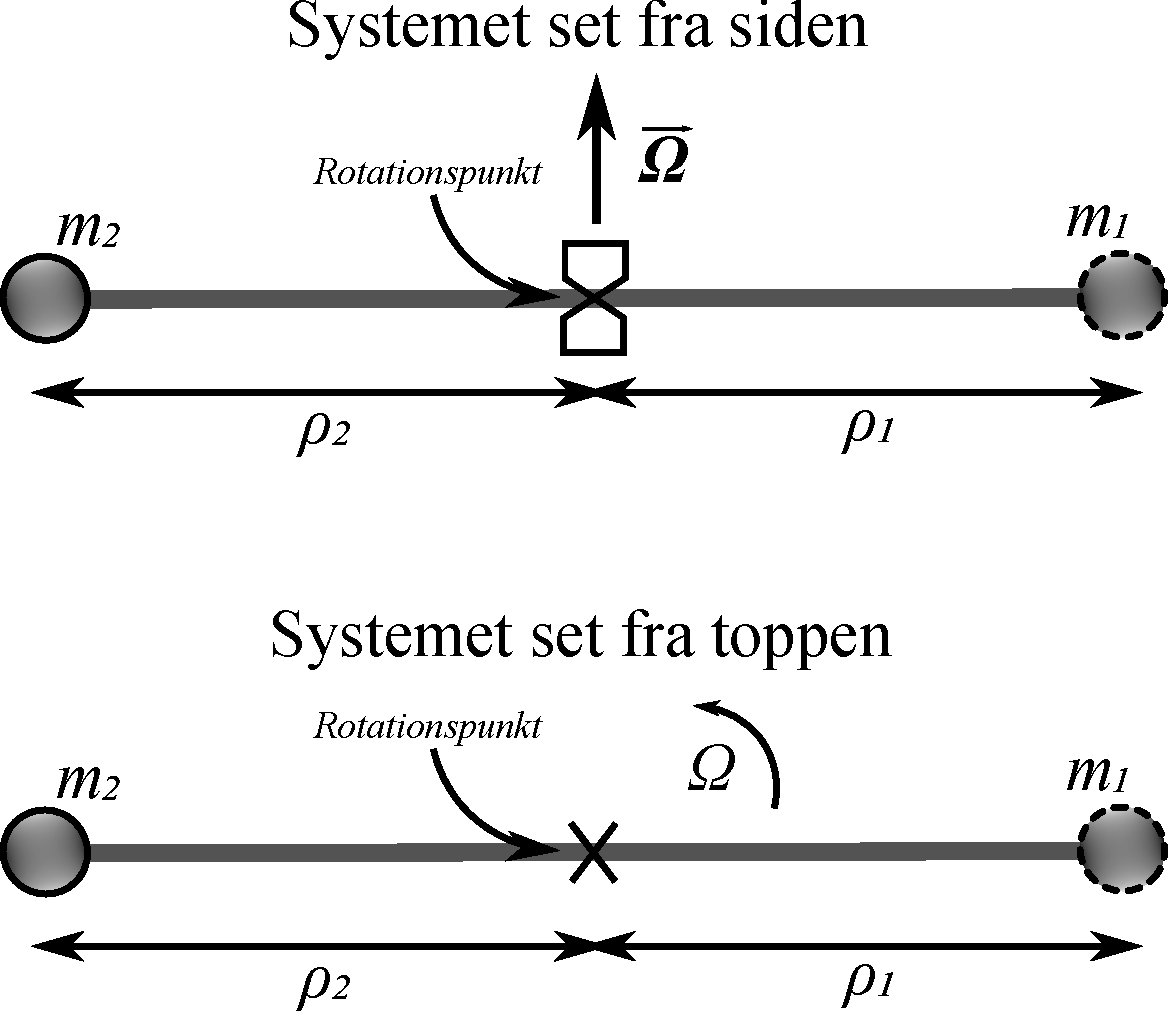
\includegraphics[width=.67\textwidth]{Analytisk-Mekanik/ToMasserRoterendeStang.pdf}
	\caption{Illustration af problemet, hvor stangen kan bevæge sig lineært gennem rotationspunktet udover at rotere med konstant vinkelhastighed $\Omega$.}	\label{fig:ToMasserRoterendeStang}
\end{figure*}
%
%
\begin{opgave}{To masser på en roterende stang}{3}
To legemer med masserne $m_1$ og $m_2$ fastspændes for enden af en stang. Denne stang monteres på et apparat, således at stangen kan rotere omkring apparatet med konstant vinkelhastighed $\v{\Omega}$, samtidig med at den kan bevæge sig friktionsløs frem og tilbage gennem apparatet. Afstanden fra legemerne til apparatet kaldes hhv. $\rho_1$ og $\rho_2$, og da vil $l = \rho_1 + \rho_2$, hvor $l$ er længden af stangen. Opstillingen kan ses på figur~\ref{fig:ToMasserRoterendeStang}.
\opg Identificer et logisk koordinatsystem at beskrive problemet i.
\opg Identificer de(n) generaliserede koordinat(er) for hvert legeme.
\opg Antagelserne giver en begrænsning af hvordan de to legemer kan bevæge sig i forhold til hinanden. Hvad er sammenhængen mellem de to legemers hastighed?
\opg Med henvisning til ligning \eqref{k-eq:FiktiveKraefter} i kompendiet bestem Coriolis og centrifugalkraften på hvert legeme, og inkluder begrænsningen på hastighederne.
\opg Tegn kræfterne der virker på hvert legeme, og beskriv hvilke antagelse tegningen bygger på.
\opg Argumenter for at Corioliskraften er ubetydelig for problemet grundet antagelserne.
\opg Benyt at summen af kræfter på et legeme i ligevægt er nul, $\sum\v{F} = \v{0}$, til at bestemme et systemets ligevægtskonfiguration.
\opg Hvordan forventes ligevægtskonfigurationen at se ud, under antagelse af at $m_1 = m_2$.
\opg Stemmer forventningen og det beregnede udtryk overens?
\end{opgave}
%
%
\begin{opgave}{Er fiktive kræfter trælse?}{3}
Betragt nu de fiktive kræfter, som givet i ligning \eqref{k-eq:FiktiveKraefter} i kompendiet.
\opg Afhænger hver af de fiktive kræfter af sted eller hastighed?
\opg Det er bøvlet, hvis eksempelvis funktionen indgår som sig selv, samt sin første og anden afledede. Med tanke på hvad de kræfter, der er arbejdet mest med i kapitlet, giver nogle af de fiktive kræfter så anledning til differentialligninger, der er specielt vanskelige at løse?
\opg Hvis differentialligningen kan skrives på formen
\begin{align*}
\dif[2]{t}{f(t)} = k\dif{t}{f(t)}
\end{align*}
kan den relativt simpelt løses. Hvorfor?
\end{opgave}
%
%
\section*{Perspektiverende Problemer}
%
%
\begin{opgave}{Tennis Racket Theorem}{4}
Indtil videre har vi kun kigget på rotationer om én akse, men ofte roterer ting om flere akser, hvilket komplicerer tingene en hel del. I denne opgave vil vi ikke forsøge at udlede bevægelsesligningerne for et sådant system, men forsøge at forstå hvilken information de kan give os. Det kan vises at bevægelsesligningerne for et stift legeme, der kan rotere om tre akser med hver sit inertimoment er
\begin{align*}
	I_x\dt{\omega}_x &= (I_y-I_z)\omega_y\omega_z \: , \\
	I_y\dt{\omega}_y &= (I_z-I_x)\omega_z\omega_x \: , \\
	I_z\dt{\omega}_z &= (I_x-I_y)\omega_x\omega_y \: ,
\end{align*}
eller på vektorform
\begin{align} \label{eq:TRT_DiffLign}
	\xyz{I_x\dt{\omega}_x}{I_y\dt{\omega}_y}{I_z\dt{\omega}_z} = \xyz{(I_y-I_z)\omega_y\omega_z}{(I_z-I_x)\omega_z\omega_x}{(I_x-I_y)\omega_x\omega_y} \: .
\end{align}
Her er $I_i$ og $\omega_i$ henholdsvis inertimomentet og vinkelhastigheden for rotation om den $i$'te akse, og yderligere antages det at $I_x>I_y>I_z>0$.
\opg Antag at $\omega_y \approx \omega_z$ er meget små og brug dette til at vise, at
\begin{align} \label{eq:TRT_DiffLignX}
	\dif{t}{}\xyz{I_x\dt{\omega}_x}{I_y\dt{\omega}_y}{I_z\dt{\omega}_z} \simeq \xyz{0}{(I_z-I_x)\dt{\omega_z}\omega_x}{(I_x-I_y)\omega_x\dt{\omega}_y} \: .
\end{align}
Hint: $\omega_y$ og $\omega_z$ er så små, at andenordensled med dem, dvs. led på formen $\omega_i\omega_j$ hvor $i=y,z$ og $j=y,z$, er nul, mens førsteordensled ikke er.
\opg Vis ved brug af ligningerne \eqref{eq:TRT_DiffLign} og \eqref{eq:TRT_DiffLignX}, at
\begin{align} \label{eq:TRT_DDiffLignX}
	\dif{t}{}\xyz{I_x\dt{\omega}_x}{I_y\dt{\omega}_y}{I_z\dt{\omega}_z} \simeq \xyz{0}{\omega_x^2\omega_y(I_z-I_x)(I_x-I_y)/I_z}{\omega_x^2\omega_z(I_x-I_y)(I_z-I_x)/I_y} \: .
\end{align}
\opg Konkluder ud fra ligning \eqref{eq:TRT_DDiffLignX} at fortegnet for $\ddt{\omega}_y$ og $\ddt{\omega}_z$ er modsat af henholdsvis $\omega_y$ og $\omega_z$.
\opg Antag nu at $\omega_x \approx \omega_z$ er meget små, analogt til spørgsmål 1), og brug helt samme metode til at vise, at
\begin{align} \label{eq:TRT_DiffLignY}
	\dif{t}{}\xyz{I_x\dt{\omega}_x}{I_y\dt{\omega}_y}{I_z\dt{\omega}_z} \simeq \xyz{\omega_y^2\omega_x(I_y-I_z)(I_x-I_y)/I_z}{0}{\omega_y^2\omega_z(I_x-I_y)(I_y-I_z)/I_x} \: .
\end{align}
\opg Benyt nu ligning \eqref{eq:TRT_DiffLignY} til at konkludere, at fortegnene for $\ddt{\omega}_x$ og $\omega_x$ er ens og ligeledes for $\omega_z$.
\opg Legemet sættes til at rotere om sin $i$'te akse, hvor vinkelhastigheden om de andre akser er små. Hvis legemet fortsætter med stort set kun at rotere om den $i$'te akse, da betragtes rotation om den $i$'te rotationsakse som stabil. Argumenter for at rotation om den $i$'te rotationsakse er stabil, hvis $\ddt{\omega}_j \propto - \omega_j \, \forall \, j\neq i$.
\opg Ved analoge udregninger fås, at $\ddt{\omega}_x \propto -\omega_x$ og $\ddt{\omega}_y \propto -\omega_y$ hvis $\omega_x\approx\omega_y$ er små. Konkluder at rotation om $x$- og $z$-aksen er stabil, mens rotation om $y$-aksen er ustabil. Dette resultat kaldes \textit{Tennis Racket Theorem}, \textit{Intermediate Axis Theorem} eller \textit{Dzhanibekov Effect}\footnote{Løses differentialligningen i ligning \ref{eq:TRT_DiffLign} fås en bevægelse som denne: \url{https://www.youtube.com/watch?v=1n-HMSCDYtM}} efter Dzhanibekov, der bemærkede det under en mission i rummet.
\opg Den eneste antagelse der er lavet, er at legemet er stift\footnote{Det er også antaget at legemet ikke er påvirket af ydre kræfter i udledningen af ligning \ref{eq:TRT_DiffLign}, men det betyder bare at konklusionen om stabilitet af rotationsakser ikke afhænger af nogle ydre kræfter.}. Brug dette til at undersøge dette fænomen med virkelige objekter, forklar hvilke rotationsakser, der er mulige for objektet, samt den relative størrelse af inertimomentet for rotation omkring de forskellige akser.
\end{opgave}
%
%
\begin{opgave}{Hamiltonfunktionen og et systems energi}{3} \label{opg:HamiltonEnergi}
Antag at et systems kinetiske energi kan skrives på formen $K = \frac{1}{2}A(q)\dt{q}^2$, hvor $A(q)$ er en arbitrær funktion af $q$, som er det eneste generaliserede koordinat. Den potentielle energi kaldes $V(q)$, og der antages kun, at den er stedsafhængig.
\opg Opskriv systemets Lagrangefunktion.
\opg Bestem den generaliserede impuls ud fra dennes definition.
\opg Udtryk $\dt{q}$ ved $p$ og $A(q)$.
\opg Benyt definitionen af Hamiltonfunktion til at bestemme denne.
\opg Vis at hvis et systems kinetiske energi kan skrives på formen $K = \frac{1}{2}A(q)\dt{q}^2$, så er $H = E$.
\opg Argumenter for at disse argumenter generaliserer til $n$ generaliserede koordinater, hvor den kinetisk energi på tilsvarende vis antages at være
\begin{align*}
	K = \sum_i\frac{1}{2}A(q_i)\dt{q}_i^2 \: .
\end{align*}
\end{opgave}
%
%
\begin{opgave}{Fra klassisk mekanik til kvantemekanik}{3}
Her vil sammenhængen mellem klassisk mekanik og kvantemekanik belyses gennem en metode til at opskrive Hamiltonoperatoren for et system, ved at starte med en klassisk analyse af problemet. Der kigges her på én partikel.
\opg Antag at den generaliserede impuls kan skrives på formen $p = m\dt{q}$. Benyt dette til at opskrive den kinetiske energi udtrykt ved impulsen $p$.
\opg Benyt resultatet fra opgave \ref{opg:HamiltonEnergi} til at opskrive systemets Hamiltonfunktion.
\opg For at kunne beskrive systemet kvantemekanisk, skal Hamiltonfunktionen skrives om til en Hamiltonoperator. Hvilke elementer i Hamiltonfunktionen skal omskrives, for at stå på operatorform?
\opg Omskriv de før angivne elementer til operatorform ved hjælp af tabel \ref{k-tab:operatorer_i_kvant} i kompendiet, og bestem derved Hamiltonoperatoren.
\end{opgave}
%
%
\begin{opgave}{Energibevarelse i Hamilton}{4}
I opgave \ref{opg:HamiltonEnergi} blev det vist at Hamiltonfunktionen i nogle tilfælde er lig med et systems energi. Det kunne derfor være interessant at undersøge, under hvilke omstændigheder Hamiltonfunktionen er bevaret over tid.
\opg Beskriv forskellen på den fuldstændige differentiation, f.eks. $\d/\d t$, og den partielle differentiation, eksempelvis $\partial/\partial t$. \footnote{Differentialoperatorerne er her skrevet med hensyn til tid, men det er bare for at give et eksempel. Der tænkes her på den generelle forskel.} 
\opg Opskriv den fuldstændigt tidsafledede af en generel Hamiltonfunktion af ét generaliseret koordinat, $\d H/\d t$, vha. kædereglen.
\opg Benyt nu Hamiltons ligninger til at simplificere summen.
\opg Konkluder at
\begin{align*}
\dif{t}{H} = \pdif{t}{H} \: .
\end{align*}
\opg Under hvilke omstændigheder er Hamiltonfunktionen bevaret i tid?
\opg Med henvisning til opgave \ref{opg:HamiltonEnergi}, hvad betyder det fysisk for systemet, at Hamiltonfunktionen er bevaret i tid?
\opg Opskriv $\d H/\d t$ for en generel Hamiltonfunktion af $n$ generaliserede koordinater, og vis at ovenstående er sandt for $n$ generaliserede koordinater.
\end{opgave}